For our strategy to be successfully applied to bytecodes corresponding
to an SCJ program, it must meet some basic requirements that ensure it
is well-formed.
Firstly, the program must pass JVM bytecode verification.
This means it must be type-correct and that execution remains inside
the array of bytecode instructions for each method.
This can be checked before execution of the program and there has
already been much work on formal verification of bytecode
verifiers~\cite{coglio2000,klein2003,xavier2003}.

Secondly, since SCJ does not allow dynamic class loading, all required
classes and methods must be present before execution of the program.
This means that the $cs$ map provided as input to the CEE must contain
all the classes referenced by any other class in $cs$.
All the bytecode instructions required for these classes must also be
present in the $bc$ map.
Our CEE model diverges if any of these requirements is not met, so
these requirements hold for any SCJ program that executes correctly in
our SCJVM interpreter.

Thirdly, due to the nature of the applications that SCJ is aimed at,
it is important that they have a structure that is readable and
facilitates verification.
MISRA-C includes such a restriction on structure and, since we are
generating C code for a safety-critical application, we aim to produce
code that is compatible with MISRA-C.
This means that the SCJ bytecode program used as input to the strategy
must also have a control structure compatible with the requirements of
MISRA-C.

\begin{figure}
  \begin{subfigure}{0.26\textwidth}
    \begin{center}
      \begin{tikzpicture}
        \useasboundingbox (-0.5,-1) rectangle (0.5,2);
        \node at (0,1.7) (start) {};
        \node at (0,1)  (A) {$\bullet$};
        \node at (0,-1) (B) {$\bullet$};
        \draw[-latex] (start) -- (A);
        \draw[-latex] (A) -- (B);
      \end{tikzpicture}
    \end{center}
    \caption{sequential composition}
    \label{sequence-figure}
  \end{subfigure}
  \begin{subfigure}{0.22\textwidth}
    \begin{center}
      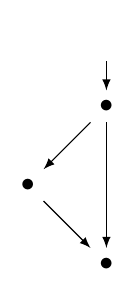
\begin{tikzpicture}
        \useasboundingbox (-1,-1) rectangle (0,2);
        \node at (0,1.7) (start) {};
        \node at (0,1)  (A) {$\bullet$};
        \node at (-1,0) (B) {$\bullet$};
        \node at (0,-1) (C) {$\bullet$};
        \draw[-latex] (start) -- (A);
        \draw[-latex] (A) -- (B);
        \draw[-latex] (A) -- (C);
        \draw[-latex] (B) -- (C);
      \end{tikzpicture}
    \end{center}
    \caption{\texttt{if} conditional}
    \label{if-figure}
  \end{subfigure}
  \begin{subfigure}{0.23\textwidth}
    \begin{center}
      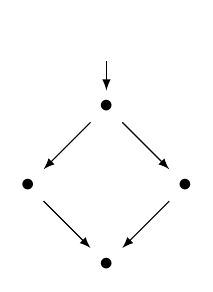
\begin{tikzpicture}
        \useasboundingbox (-1,-1) rectangle (1,2);
        \node at (0,1.7) (start) {};
        \node at (0,1)  (A) {$\bullet$};
        \node at (1,0)  (B) {$\bullet$};
        \node at (-1,0) (C) {$\bullet$};
        \node at (0,-1) (D) {$\bullet$};
        \draw[-latex] (start) -- (A);
        \draw[-latex] (A) -- (B);
        \draw[-latex] (A) -- (C);
        \draw[-latex] (B) -- (D);
        \draw[-latex] (C) -- (D);
      \end{tikzpicture}
    \end{center}
    \caption{\texttt{if}-\texttt{else} conditional}
    \label{if-else-figure}
  \end{subfigure}
  \begin{subfigure}{0.25\textwidth}
    \begin{center}
      \begin{tikzpicture}
        \useasboundingbox (-1,0) rectangle (1,3);
        \node at (0,1.7) (start) {};
        \node at (0,1)  (A) {$\bullet$};
        \node at (1,0)  (B) {$\bullet$};
        \node at (-1,0) (C) {$\bullet$};
        \draw[-latex] (start) -- (A);
        \draw[-latex] (A) -- (B);
        \draw[-latex] (A) -- (C);
      \end{tikzpicture}
    \end{center}
    \caption{divergent conditional}
    \label{divergent-figure}
  \end{subfigure} 
  \\
  \begin{subfigure}{0.32\textwidth}
    \begin{center}
      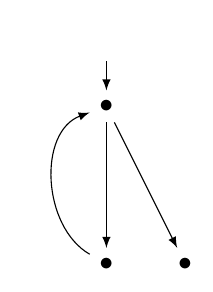
\begin{tikzpicture}
        \useasboundingbox (-1,-1) rectangle (1,2);
        \node at (0,1.7) (start) {};
        \node at (0,1) (A) {$\bullet$};
        \node at (0,-1) (B) {$\bullet$};
        \node at (1,-1) (C) {$\bullet$};
        \draw[-latex] (start) -- (A);
        \draw[-latex] (A) to (B);
        \draw[-latex] (A) to (C);
        \draw[-latex] (B) to[in=200,out=150] (A);
      \end{tikzpicture}
    \end{center}
    \caption{\texttt{while} loop}
    \label{while-figure}
  \end{subfigure}
  \begin{subfigure}{0.32\textwidth}
    \begin{center}
      \begin{tikzpicture}
        \useasboundingbox (-1,0) rectangle (1,3);
        \node at (0,1.7) (start) {};
        \node at (0,1)  (A) {$\bullet$};
        \node at (1,0)  (B) {$\bullet$};
        \draw[-latex] (start) -- (A);
        \draw[-latex] (A) to (B);
        \draw[-latex] (A) to[out=235,in=180,looseness=10] (A);
      \end{tikzpicture}
    \end{center}
    \caption{\texttt{do}-\texttt{while} loop}
    \label{do-while-figure}
  \end{subfigure}
  \begin{subfigure}{0.32\textwidth}
    \begin{center}
      \begin{tikzpicture}
        \useasboundingbox (-1,0) rectangle (1,3);
        \node at (0,1.7) (start) {};
        \node at (0,1)  (A) {$\bullet$};
        \draw[-latex] (start) -- (A);
        \draw[-latex] (A) to[out=270,in=180,looseness=10] (A);
      \end{tikzpicture}
    \end{center}
    \caption{infinite loop}
    \label{infinite-loop-figure}
  \end{subfigure}
  \caption{Control flow graphs of program structures}
  \label{structured-cfg-figures}
\end{figure}

Precisely, we require the control flow graph of each method in the
input program to have a structure based on Dijkstra's notion of
program structure found in~\cite{dijkstra1972}.
In our definition of a structured program, the control flow graph must
be composed of the structures shown in
Figure~\ref{structured-cfg-figures}. 
The first structure (Figure~\ref{sequence-figure}) is that of simple
sequential composition, with an edge going from the root node to a
single end node.
The next three structures
(Figure~\ref{if-figure}--\subref{divergent-figure}) are conditional
structures. 
Figure~\ref{if-figure} shows an \texttt{if} statement with no
\texttt{else} clause. 
Figure~\ref{if-else-figure} shows an \texttt{if} statement with an
\texttt{else} clause. 
Figure~\ref{divergent-figure} shows a conditional in which both
branches end with a (infinite) loop or a return so that there is
nothing following the conditional; we refer to such conditionals as
divergent conditionals since the branches do not come back together.
The remaining three structures
(Figure~\ref{while-figure}--\subref{infinite-loop-figure}) are all
loops.
Figure~\ref{while-figure} shows a loop in which the loop condition is
checked at the beginning (a \texttt{while} loop).
Figure~\ref{do-while-figure} shows a loop in which the loop condition
is checked at the end (a \texttt{do}-\texttt{while} loop).
Figure~\ref{infinite-loop-figure} shows an infinite loop.

We provide below a formal definition of what it means for a control
flow graph to be structured. 
This definition is based on that in~\cite{bento2017}, which provides
an algorithm for recognising structured graphs.
We first define a rooted directed graph below. 
The definition is standard, but we include it here to introduce the
terminology for the subsequent definition.
\begin{defn}[Rooted Directed Graph] A \emph{rooted directed graph},
$G$, is a triple $(V,E,r)$, where
  \begin{itemize}
  \item $V$ is a set of \emph{nodes},
  \item $E$ is a set of ordered pairs of nodes in $V$, called
\emph{edges}, and
  \item $r$ is a node in $V$, called the \emph{root} of the graph.
  \end{itemize}
  The first component of an edge is its \emph{source}
  and the second component is its \emph{target}. 
  We say that an edge goes from its source to its target. 
  For every node $n \in V$, the pair $(r,n)$ must be in the reflexive
  transitive closure of $E$, that is, there must be a path of edges
  from the root to any node in the graph.
  For a graph $G$, we refer to the set
  $T(G) = \{ n \in V | \forall m \in V.\; (n,m) \notin E\}$ of nodes
  with no edges coming from them as the set of \emph{end nodes} of the
  graph.
\end{defn}
In diagrams we represent the nodes as points or as the names of the
nodes, the edges as arrows, and the root node as a node with an arrow
pointing to it that does not come from another node.
Additionally, we refer to the source of an edge going to a given node
as a \emph{predecessor} of that node; similarly, the target of an edge
from a given node is a \emph{successor} of that node.

We now define what it means to replace a node in a graph by another
graph.
We use this concept to construct more complex structured graphs from
those shown in Figure~\ref{structured-cfg-figures}.
Node replacement may occur in four different ways, depending on which
node is being replaced in a graph.
We illustrate the different cases of node replacement using the
example graphs $G$ and $H$ shown in Figure~\ref{G-H-examples-figure}.
The $G$ graph has the form of a conditional with two branches, and the
$H$ graph has the form of a \texttt{while} loop.
We label the nodes of the graphs separately for ease of reference.

\begin{figure}
  \begin{center}
    \begin{tikzpicture}
      \useasboundingbox (-3,-2) rectangle (2,2);
      \node at (-1,2) {$G$};
      \node at (0,1.7) (start) {};
      \node at (0,1)  (A) {$1$};
      \node at (1,0)  (B) {$2$};
      \node at (-1,0) (C) {$3$};
      \node at (0,-1) (D) {$4$};
      \draw[-latex] (start) -- (A);
      \draw[-latex] (A) -- (B);
      \draw[-latex] (A) -- (C);
      \draw[-latex] (B) -- (D);
      \draw[-latex] (C) -- (D);
    \end{tikzpicture}
    \begin{tikzpicture}
      \useasboundingbox (-3,-2) rectangle (2,2);
      \node at (-1,2) {$H$};
      \node at (0,1.7) (start) {};
      \node at (0,1) (A) {$a$};
      \node at (0,-1) (B) {$b$};
      \node at (1,-1) (C) {$c$};
      \draw[-latex] (start) -- (A);
      \draw[-latex] (A) to (B);
      \draw[-latex] (A) to (C);
      \draw[-latex] (B) to[in=200,out=150] (A);
    \end{tikzpicture}
    \caption{Example control flow graphs to illustrate node
      replacement}
    \label{G-H-examples-figure}
  \end{center}
\end{figure}

The first case is that of placing a graph at the start of another
graph, i.e.\ replacing the root node of a graph that does not have a
loop to its root node.
An example of this can be seen in
Figure~\ref{root-replacement-figure}, where the root node (node $1$)
of graph $G$ is replaced with graph $H$.
The unique end node of graph $H$, node $c$, takes the place of node
$1$.
The other nodes of $H$ are connected to it by the same edges as in
$H$.

The second case is that of replacing one of the end nodes of a graph.
This is shown in Figure~\ref{end-replacement-figure}, where node $4$
of graph $G$ is replaced with graph $H$.
Node $a$, the root node of graph $H$, takes the place of node $4$.
As in the previous case, the remaining nodes of $H$ are included,
connected to $a$ by the same edges as in $H$.

The third case (Figure~\ref{internal-replacement-figure}) is that of
replacing an internal node of the graph.
In our example, node $2$ of graph $G$ is replaced with graph $H$.
There is an edge from the predecessor of node $2$, which is node $1$
in this case, to the root node of $H$ (node $a$).
There is another edge from the end node of $H$ (node $c$), which is
required to be unique, to the successor of node $3$, which is node $4$
in this case.

The final case, an example of which is shown in
Figure~\ref{branch-end-replacement-figure}, is where control flow
constructs occur at the end of one branch of a conditional.
In our example, node $2$ of graph $G$ is replaced with graph $H$, as
in the previous case, but the end node of $H$ (node $c$) is identified
with the successor of node $2$ (node $4$), and so it is not included
in the graph.
Thus, this represents the case in which no instructions occur inside
the conditional branch after the while loop.
Such instructions are represented by node $c$ in
Figure~\ref{internal-replacement-figure}, which is excluded in
Figure~\ref{branch-end-replacement-figure}.

\begin{figure}
  \begin{subfigure}{0.24\textwidth}
    \begin{center}
      \begin{tikzpicture}
        \useasboundingbox (-1.5,-2.5) rectangle (1.5,2);
        \node at (0,2) (start) {};
        \node at ( 0, 1)  (A) {$a$};
        \node at (-1, 0)  (B) {$b$};
        \node at ( 0,0)   (D) {$c$};
        \node at (-1,-1)  (E) {$2$};
        \node at ( 1,-1)  (F) {$3$};
        \node at ( 0,-2)  (G) {$4$};
        \draw[-latex] (start) -- (A);
        \draw[-latex] (A) to (B);
        \draw[-latex] (A) to (D);
        \draw[-latex] (B) to[in=180,out=90] (A);
        \draw[-latex] (D) -- (E);
        \draw[-latex] (D) -- (F);
        \draw[-latex] (E) -- (G);
        \draw[-latex] (F) -- (G);
      \end{tikzpicture}
    \caption{\centering root node\newline replacement}
    \label{root-replacement-figure}
  \end{center}
  \end{subfigure}
  \begin{subfigure}{0.24\textwidth}
    \begin{center}
      \begin{tikzpicture}
        \useasboundingbox (-1.5,-2.5) rectangle (1.5,2);
        \node at (0,2) (start) {};
        \node at ( 0, 1)  (A) {$1$};
        \node at (-1, 0)  (B) {$2$};
        \node at ( 1, 0)  (C) {$3$};
        \node at ( 0,-1)  (D) {$a$};
        \node at ( 0,-2)  (E) {$b$};
        \node at ( 1,-2)  (F) {$c$};
        \draw[-latex] (start) -- (A);
        \draw[-latex] (A) -- (B);
        \draw[-latex] (A) -- (C);
        \draw[-latex] (B) -- (D);
        \draw[-latex] (C) -- (D);
        \draw[-latex] (D) to (E);
        \draw[-latex] (D) to (F);
        \draw[-latex] (E) to[in=200,out=150] (D);
      \end{tikzpicture}
    \caption{\centering end node\newline replacement}
    \label{end-replacement-figure}
    \end{center}
  \end{subfigure}
  \begin{subfigure}{0.24\textwidth}
    \begin{center}
      \begin{tikzpicture}
        \useasboundingbox (-1.5,-2.5) rectangle (1.5,2);
        \node at (0,2) (start) {};
        \node at ( 0, 1)    (A) {$1$};
        \node at (-1, 0)    (B) {$a$};
        \node at ( 1,-0.5)  (C) {$3$};
        \node at (-2,-1)    (D) {$b$};
        \node at (-1,-1)    (F) {$c$};
        \node at ( 0,-2)    (G) {$4$};
        \draw[-latex] (start) -- (A);
        \draw[-latex] (A) -- (B);
        \draw[-latex] (A) -- (C);
        \draw[-latex] (B) to (D);
        \draw[-latex] (B) to (F);
        \draw[-latex] (D) to[in=180,out=90] (B);
        \draw[-latex] (F) -- (G);
        \draw[-latex] (C) -- (G);
      \end{tikzpicture}
      \caption{\centering internal node\newline replacement}
      \label{internal-replacement-figure}
    \end{center}
  \end{subfigure}
  \begin{subfigure}{0.24\textwidth}
    \begin{center}
      \begin{tikzpicture}
        \useasboundingbox (-1.5,-2.5) rectangle (1.5,2);
        \node at (0,2) (start) {};
        \node at ( 0, 1)    (A) {$1$};
        \node at (-1,-0.5)  (B) {$a$};
        \node at ( 1,-0.5)  (C) {$3$};
        \node at (-2,-1.5)  (D) {$b$};
        \node at ( 0,-2)    (G) {$4$};
        \draw[-latex] (start) -- (A);
        \draw[-latex] (A) -- (B);
        \draw[-latex] (A) -- (C);
        \draw[-latex] (B) to (D);
        \draw[-latex] (B) to (G);
        \draw[-latex] (D) to[in=180,out=90] (B);
        \draw[-latex] (C) -- (G);
      \end{tikzpicture}
    \caption{\centering branch end\newline replacement}
    \label{branch-end-replacement-figure}
  \end{center}
  \end{subfigure}
  \caption{Examples of the different cases of node replacement}
  \label{node-replacement-example-figures}
\end{figure}

In general, we define node replacement using the formal definition
below.
This covers each of the four cases shown above.
\begin{defn}[Node Replacement]
  Given two rooted directed graphs $G$ and $H$, we say $G'$ is the
  graph formed by \emph{replacing} a node $n$ of $G$ with $H$ if one
  of the following cases holds:
  \begin{itemize}
  \item $n$ has no predecessors in $G$, $H$ has only one end node, and
    \begin{itemize}
    \item $G'$ contains all the nodes of $H$ and $G$, except $n$,
    \item $G'$ contains the edges of $G$ and the edges of $H$ except
      those going to or from $n$,
    \item $G'$ contains edges from the end node of $H$ to the
      successors of $n$ in $G$, and
    \item the root node of $G'$ is the root node of $H$;
    \end{itemize}
  \item $n$ has no successors in $G$, $n$ is not the root node of $G$, and
    \begin{itemize}
    \item $G'$ contains all the nodes of $H$ and $G$, except $n$,
    \item $G'$ contains the edges of $G$ and the edges of $H$ except
      those going to or from $n$,
    \item $G'$ contains edges from the predecessors $n$ in $G$ to the
      root node of $H$, and
    \item the root node of $G'$ is the root node of $G$;
    \end{itemize}
  \item $H$ has a single end node, $n$ is not the root node or an end
    node of $G$, and
    \begin{itemize}
    \item $G'$ contains all the nodes of $H$ and $G$, except $n$,
    \item $G'$ contains the edges of $G$ and the edges of $H$ except
      those going to or from $n$,
    \item $G'$ contains edges from the predecessors of $n$ in $G$ to
      the root node of $H$,
    \item $G'$ contains edges from the end node of $H$ to the
      successors of $n$ in $G$, and
    \item the root node of $G'$ is the root node of $G$;
    \end{itemize}
  \item $n$ has a single successor in $G$, $n$ is not the root node of
    $G$, $H$ has a single end node, and
    \begin{itemize}
    \item $G'$ contains all the nodes of $H$ and $G$, except $n$ and
      the end node of $H$,
    \item $G'$ contains the edges of $G$ and the edges of $H$ except
      those going to or from $n$ or the end node of $H$,
    \item $G'$ contains edges from the predecessors of the end node of
      $H$ to the successor of $n$ in $G$
    \item $G'$ contains edges from the predecessors of $n$ in $G$ to
      the root node of $H$, and
    \item the root node of $G'$ is the root node of $G$.
    \end{itemize}
  \end{itemize}
\end{defn}

With node replacement defined, we can now finally define what we mean
by a structure control flow graph in terms of node replacement and the
structured graphs shown in Figure~\ref{structured-cfg-figures}

\begin{defn}[Structured Control Flow Graph]
  If $G$ is a rooted directed graph, we say $G$ is a \emph{structured
    control flow graph} if $G$ is the trivial graph (the graph with a
  single node, which is also the root, and no edges) or if $G$ can be
  created by starting with the trivial graph and performing a finite
  number of node replacements to replace nodes with graphs of the
  forms shown in Figure~\ref{structured-cfg-figures}.
\end{defn}

Before applying the strategy, it must be ensured that the control flow
graph for each method is well-structured according to this definition.

We also require that integer operations are used only where integer
overflow cannot occur.
This is due to the fact that we follow icecap's approach and compile
addition in Java bytecode to addition in C, making the assumption that
the addition does not overflow, since overflow is undefined behaviour
in C.
The Java code should be written in a style consistent with MISRA-C,
where behaviours that are undefined in C must not be relied on.

We do not handle synchronisation of static methods, since icecap does
not apply synchronisation to static methods.
It is important that we follow the approach of a practical tool on
this, to ensure that our strategy can be implemented.
No expressive power is lost by forbidding static synchronized methods,
since a singleton instance of a class with synchronized methods can be
supplied, rather than relying on static methods to access data owned
by the instance.

Each method call must have at least one target (as
determined by the rules given in
Section~\ref{resolve-method-calls-subsection}), to allow method calls
to be resolved.
Each \texttt{invokestatic} and \texttt{invokespecial} instruction has
exactly one target, so this poperty is always fulfilled for such
method calls.
For \texttt{invokevirtual} instructions, a method call only has no
targets if the method in which the instruction occurs is unused or if
the method is invoked on a null pointer (which is erroneous).
Methods not used in the program should not be included in the
parameters passed to $CEE$, matching icecap's behaviour of excluding
such methods from the generated code.

Finally, we require that no method in the program recurses, either
directly or indirectly.
This is because recursion is not recommended in safety-critical
applications because of the potential for unpredictable failure due to
stack overflow, and it is not allowed in MISRA-C for that reason.
Imposing this requirement allows us to handle methods individually
when introducing their control flow, without considering circular
dependencies between them.

We now proceed to describe each of the stages of the strategy in
detail, beginning with the \emph{Elimination of Program Counter} stage
in the next section.